% One action's cost divided along a saturated chain, and what is left over.
\documentclass[tikz,border=0pt]{standalone}
\usepackage{amsmath}
\usepackage{tikz}
\usetikzlibrary{backgrounds,arrows.meta,positioning,decorations.pathreplacing}
\definecolor{hdblue}{HTML}{1B4F8A}
\definecolor{hdred}{HTML}{A62B1F}
\definecolor{hdgrey}{HTML}{6B7280}
\begin{document}
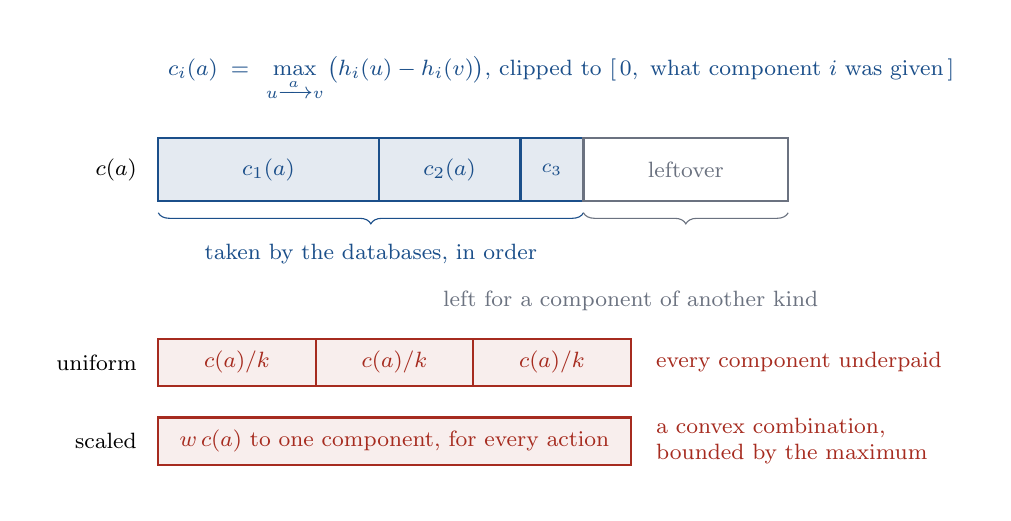
\begin{tikzpicture}[
    show background rectangle, inner frame sep=7pt,
    background rectangle/.style={fill=white},
    font=\footnotesize, >={Latex[length=4pt]}]

  \node[anchor=west,align=left,hdblue] at (0, 1.55)
       {$c_i(a) \;=\; \displaystyle\max_{\,u \xrightarrow{\,a\,} v\,}
        \bigl( h_i(u) - h_i(v) \bigr)$,
        clipped to $[\,0,\ \text{what component } i \text{ was given}\,]$};

  % --- the saturated chain: one action's cost, divided
  \node[anchor=east] at (-0.15, 0.4) {$c(a)$};
  \fill[hdblue!12] (0,0) rectangle (5.4,0.8);
  \draw[hdblue,thick] (0,0) rectangle (2.8,0.8);
  \draw[hdblue,thick] (2.8,0) rectangle (4.6,0.8);
  \draw[hdblue,thick] (4.6,0) rectangle (5.4,0.8);
  \draw[hdgrey,thick] (5.4,0) rectangle (8.0,0.8);
  \node[hdblue] at (1.4,0.4) {$c_1(a)$};
  \node[hdblue] at (3.7,0.4) {$c_2(a)$};
  \node[hdblue,font=\scriptsize] at (5.0,0.4) {$c_3$};
  \node[hdgrey] at (6.7,0.4) {leftover};

  \draw[decorate,decoration={brace,amplitude=4pt,mirror},hdblue]
        (0,-0.15) -- (5.4,-0.15);
  \draw[decorate,decoration={brace,amplitude=4pt,mirror},hdgrey]
        (5.4,-0.15) -- (8.0,-0.15);
  \node[hdblue,anchor=north] at (2.7,-0.42) {taken by the databases, in order};
  \node[hdgrey,anchor=north] at (6.0,-1.02) {left for a component of another kind};

  % --- the two schemes it is not, for contrast
  \node[anchor=east] at (-0.15,-2.05) {uniform};
  \draw[hdred,thick,fill=hdred!8] (0,-2.35) rectangle (2.0,-1.75);
  \draw[hdred,thick,fill=hdred!8] (2.0,-2.35) rectangle (4.0,-1.75);
  \draw[hdred,thick,fill=hdred!8] (4.0,-2.35) rectangle (6.0,-1.75);
  \node[hdred] at (1.0,-2.05) {$c(a)/k$};
  \node[hdred] at (3.0,-2.05) {$c(a)/k$};
  \node[hdred] at (5.0,-2.05) {$c(a)/k$};
  \node[anchor=west,hdred] at (6.2,-2.05) {every component underpaid};

  \node[anchor=east] at (-0.15,-3.05) {scaled};
  \draw[hdred,thick,fill=hdred!8] (0,-3.35) rectangle (6.0,-2.75);
  \node[hdred] at (3.0,-3.05) {$w\,c(a)$ to one component, for every action};
  \node[anchor=west,hdred,align=left] at (6.2,-3.05) {a convex combination,\\bounded by the maximum};
\end{tikzpicture}
\end{document}
